\section{Microsoft Windows}

\subsection{Requisites}

To compile GMAC, the following software must be installed:
\begin{itemize}
\item CMake 2.8 or higher (http://www.cmake.org)
\item Visual Studio 2008 SP1
\item AMD APP SDK 2.5 or higher (http://developer.amd.com/gpu/AMDAPPSDK)
\end{itemize}

Additionally, to build the GMAC documentation, there are the following extra requisites:
\begin{itemize}
\item Doxygen (http://www.doxygen.org)
\item Miktex (http://miktex.org) with the following packages: Memoir (document class), 
graphicx, tabularx, wrapfig, listings, xspace, hyphenat, and hyperref.
\item GNOME Dia (http://projects.gnome.org/dia)
\end{itemize}

\subsection{Compilation and Installation}
First you need to extract GMAC from the zip file, which will create a directory called 
\texttt{gmac}. 

GMAC uses CMake to generate platform\hyp{}specific compilation scripts, so the CMake GUI is used to 
configure GMAC\@. Launch CMake\hyp{}GUI and set the source directory to the path where you extracted 
GMAC, and the build directory to a build subdirectory inside GMAC, as in 
Figure~\ref{fig:install:cmake-init}, and click the \emph{Configure} button.
\begin{figure}[h]
\centering
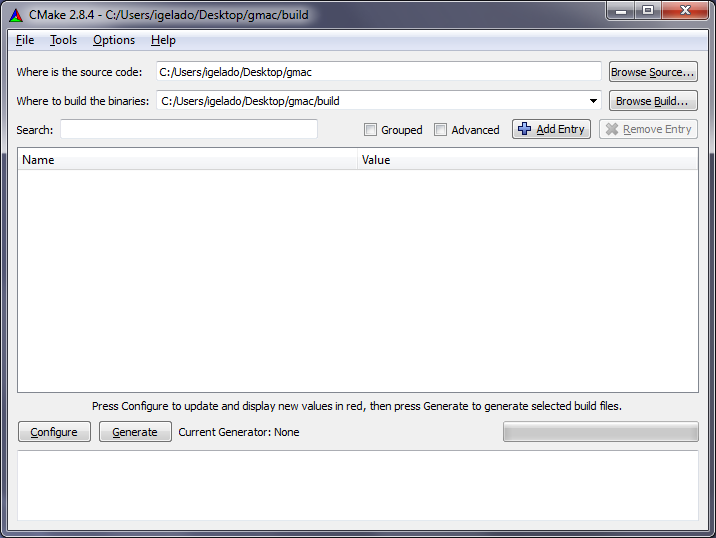
\includegraphics[width=0.8\linewidth]{installation/figures/cmake-init}
\caption{Step 1, set the source and build path in CMake\hyp{}GUI}
\label{fig:install:cmake-init}
\end{figure}

A new CMake window (Figure~\ref{fig:install:cmake-compiler}) appears to ask for the compiler to be 
used; select \emph{Visual Studio 9 2008} to compile GMAC for 32\hyp{}bits, or \emph{Visual Studio 9 
2008 Win64} to compile GMAC for 64\hyp{}bits.
\begin{figure}[h]
\centering
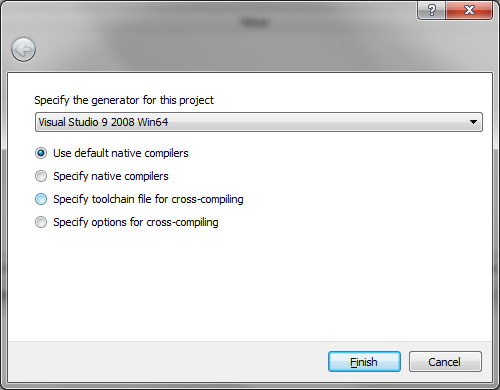
\includegraphics[width=0.6\linewidth]{installation/figures/cmake-compiler}
\caption{Step 2, select the compiler to be used}
\label{fig:install:cmake-compiler}
\end{figure}

After an initial configuration attempt, CMake will report an error 
(Figure~\ref{fig:install:cmake-conf-error}) because it fails to guess the configuration parameters 
for the system.
\begin{figure}[h]
\centering
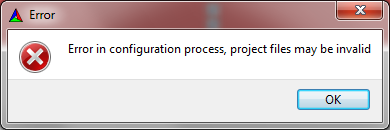
\includegraphics[width=0.5\linewidth]{installation/figures/cmake-conf-error}
\caption{Configuration error; CMake is unable to guess the configuration}
\label{fig:install:cmake-conf-error}
\end{figure}

Select \texttt{USE\_OPENCL}, and \texttt{USE\_LITE}, as in Figure~\ref{fig:install:cmake-opencl}, 
and click on \emph{Configure}.
\begin{figure}[h]
\centering
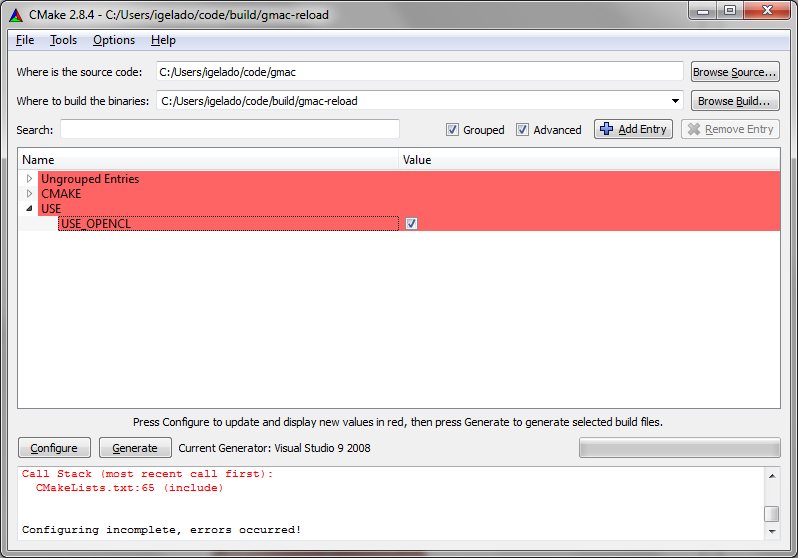
\includegraphics[width=0.8\linewidth]{installation/figures/cmake-opencl}
\caption{Step 3, set the correct configuration parameters in CMake\hyp{}GUI}
\label{fig:install:cmake-opencl}
\end{figure}

A new error window will appear (Figure~\ref{fig:install:cmake-opencl-error}) if CMake fails to find 
the location of the OpenCL header files and libraries.
\begin{figure}[h]
\centering
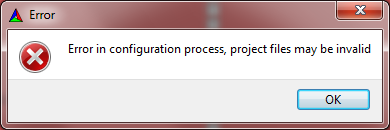
\includegraphics[width=0.5\linewidth]{installation/figures/cmake-opencl-error}
\caption{Configuration error; CMake does not find OpenCL files}
\label{fig:install:cmake-opencl-error}
\end{figure}


In such a case, you need to set those paths by hand, as in 
Figure~\ref{fig:install:cmake-opencl-path}, a click on \emph{Configure} again. Finally, a new Visual 
Studio project will be produced inside the \texttt{build} folder.
\begin{figure}[h]
\centering
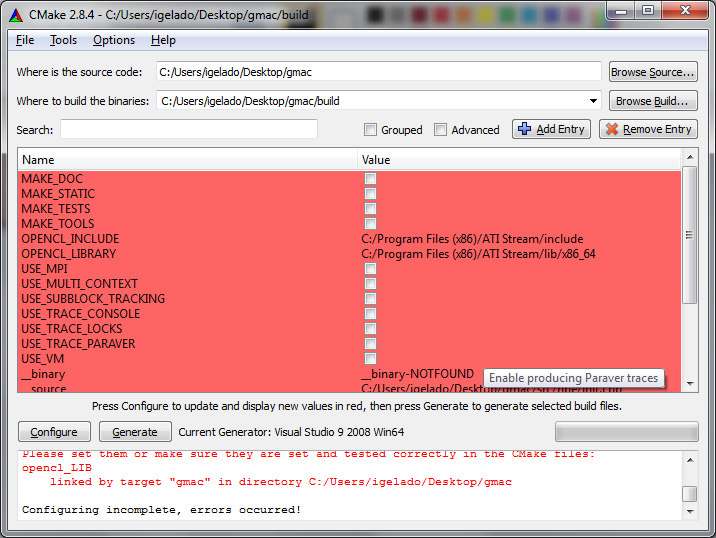
\includegraphics[width=0.8\linewidth]{installation/figures/cmake-opencl-path}
\caption{Step 4, set the path for the OpenCL header files and libraries}
\label{fig:install:cmake-opencl-path}
\end{figure}

Open the \emph{gmac} Visual Studio project, located in the \emph{build} folder inside GMAC\@. Inside 
Visual Studio, set the active configuration to \emph{Release}, and press F7 to compile GMAC\@.  
Finally, build the \texttt{INSTALL} project to install GMAC in your system.


% vim: set spell ft=tex fo=aw2t expandtab sw=2 tw=100:
